% Basic document style
\documentclass{article}
\usepackage[utf8]{inputenc}
\usepackage[margin=1in]{geometry}
\usepackage{inconsolata} % prettier texttt
\renewcommand{\familydefault}{\sfdefault}

% Graphics, tables and figures
\usepackage{enumitem}
\usepackage{hyperref}
\usepackage{float}
\usepackage[table, x11names]{xcolor}
\usepackage{graphicx}
\usepackage{listings}
\usepackage{autogobble}
\usepackage{tikz}

\lstset{
	basicstyle=\footnotesize\color{black}\ttfamily,
	belowcaptionskip=1\baselineskip,
	breaklines=true,
	xleftmargin=\parindent,
	xrightmargin=\parindent,
	showstringspaces=false,
	keywordstyle=\color{Firebrick3},
	keywordstyle=[2]\color{DodgerBlue4},
	commentstyle=\color{MistyRose4},
	stringstyle=\color{Green4},
	rulecolor=\color{black!50},
	tabsize=4,
	autogobble,
	frame=l,
	framerule=2pt
}
\lstdefinestyle{cdb}{ language=Python, rulecolor=\color{blue!50}, moredelim=[is][\color{Goldenrod4}]{<m>}{</m>}, moredelim=[s][\color{Goldenrod4}]{\$}{\$}, morekeywords={ assert }, keywords=[2]{ sym, cdb2python_string, explicit_indices, rhs, simplify, young_project, einsteinify, collect_terms, compile_package__, slot_sym, factor_in, young_project_tensor, eliminate_metric, cdb2python, init_ipython, zoom, take_match, collect_factors, slot_asym, expand_dummies, untrace, sort_sum, product_rule, lhs, split_gamma, epsilon_to_delta, rename_dummies, unwrap, decompose, eliminate_vielbein, create_scope, drop_weight, order, eliminate_kronecker, join_gamma, reduce_delta, distribute, integrate_by_parts, evaluate, rewrite_indices, expand_delta, vary, sort_spinors, asym, kernel, map_sympy, split_index, decompose_product, young_project_product, substitute, lower_free_indices, replace_match, expand_diracbar, complete, collect_components, tree, keep_weight, unzoom, meld, create_scope_from_global, terms, fierz, create_empty_scope, keep_terms, sort_product, raise_free_indices, properties, indexsort, expand, tab_dimension, expand_power, lr_tensor, canonicalise, combine, flatten_sum, factor_out, Distributable, AntiSymmetric, Accent, SelfCommutingBehaviour, WeightInherit, SelfCommuting, KroneckerDelta, AntiCommuting, Weight, Spinor, CommutingBehaviour, InverseMetric, DAntiSymmetric, SelfNonCommuting, Vielbein, Coordinate, scalar_backend_t, Diagonal, NumericalFlat, TableauInherit, Traceless, DependsBase, SortOrder, InverseVielbein, match_t, Indices, WeightBase, Derivative, WeylTensor, DifferentialFormBase, FilledTableau, CommutingAsProduct, ProgressMonitor, Tableau, CommutingAsSum, LaTeXForm, RiemannTensor, TableauSymmetry, list_property, SatisfiesBianchi, Metric, ExNode, Commuting, warn_t, TableauObserver, ExteriorDerivative, Total, Symmetric, Integer, SelfAntiCommuting, Trace, result_t, Ex, labelled_property, Stopwatch, DifferentialForm, NonCommuting, EpsilonTensor, PartialDerivative, Property, Symbol, ImaginaryI, TableauBase, IndexInherit, SympyBridge, Determinant, GammaMatrix, ImplicitIndex, Kernel, DiracBar, Matrix, Depends, parent_rel_t, } }
\lstnewenvironment{lstcdb}{\lstset{style=cdb}}{}
\lstnewenvironment{lstverb}{\lstset{moredelim=[is][\bfseries\color{Green3}]{<add>}{</add>}}}{}
\lstnewenvironment{lstlatex}{\lstset{ rulecolor=\color{Green4!50}, morekeywords={ \algorithm, \texttt } } }{}
\lstnewenvironment{lstcpp}{\lstset{ language=C++, moredelim=[is][\bfseries\color{Green3}]{<add>}{</add>}, morekeywords={override}, rulecolor=\color{LightPink2}}}{}

% Copied from the cadabra preamble.tex
\newcommand{\algorithm}[2]{{\tt\Large\detokenize{#1}}\\[1ex]
{\emph{#2}}\\[1ex]
}


% Maths 
\usepackage{amsmath}
\usepackage{amssymb}
\usepackage[vcentermath]{youngtab}

\title{Writing Algorithms in Cadabra2}
\author{Dominic Price}
\date{}

\begin{document}
\maketitle

Cadabra is a powerful computer algebra system which is specialised for handling tensor field calculations
and is built on top of Python. By using Python as a foundation, it is very easy to extend the functionality of
Cadabra with custom algorithms to perform specific tasks as well as very generic routines which can use the 
incredibly flexible and reflective language features of Python to dynamically respond to different inputs.

This is a brief introduction to writing algorithms in Cadabra, introducing some of the typical idioms which allow
user algorithms to behave like the inbuilt routines as well as the various language features and technical 
considerations of writing algorithms.

The first section is a purely Python centred guide and assumes a basic familiarity with both Cadabra and Python
with any more advanced language features being explained and external resources to provide more details linked.
In the second section, the infrastructure of the underlying C++ codebase is explained and directions on how to
extend Cadabra using C++ is covered. This is a slightly more advanced discussion although it is aimed to be
accessible for casual users of C++. 

\section{What is an algorithm in Cadabra?}

Before diving into the ins and outs of \emph{how} to write an algorithm for Cadabra, it is first worth discussing exactly
what specifically we are talking about as the term `algorithm' is quite general. For the purposes of this tutorial, when
talking about an algorithm we are specifically talking about a function which satisfies some criteria:
\begin{enumerate}
	\item The number of argument it takes can vary, but its first argument must be a \verb|Ex| object
	\item It should apply transformations on this expression
	\item It then returns a reference to this expression
\end{enumerate}
The functions in the Cadabra core all satisfy this format, and most of the functions found in the \verb|cdb.*| libraries are
too although occasionally they will instead create a copy of the input expression instead of modifying it. An example of an
algorithm which acts like this is \verb|get_component| from the \verb|cdb.core.component| library which resolves the free
indices of an expression into specified components.

While it is of course possible to write functions which modify expression and which \emph{don't} follow these
criteria, if you are planning to release your algorithm to the wider community or even are collaborating on a 
project then by making sure that you follow these requirements your code will be far more intuitive for others to
follow and will be able to be used alongside the inbuilt Cadabra algorithms seamlessly. To illustrate, the 
following function
\begin{lstcdb}
	def distribute_excluding(subex, ex):
		substitute(ex, $@(subex) -> qqq$)
		distribute(ex)
		substitute(ex, $qqq -> @(subex)$)
		return True
\end{lstcdb}
which takes the `acting' expression as a second parameter and returns a \verb|bool| is almost certain to be a common source
of bugs and look out of place in a list of algorithm calls:
\begin{lstcdb}
	...
	unwrap(ex)
	substitute(ex, $\partial_{\mu}{p} -> 0$)
	distribute_excluding($t - s$, ex)
	...
\end{lstcdb}
and also prevents users from immediately viewing the results of the algorithm:
\begin{lstcdb}
	ex := (x + y)*(a + b)*(c + d)
	substitute(ex, $a + b -> 1$); # Displays $(x+y)(c+d)$
	distribute_excluding($x + y$, ex); # Displays 'True'
\end{lstcdb}


\section{Writing Cadabra algorithms in Python}

Having covered what an algorithm is, we can now start looking at ways to implement them. Using pure Python, there
are two basic constructions which can be used for interfacing an algorithm: the simplest method is by using a 
Python function definition which satisfies the criteria given above. The second method is by using the special
\verb|@algo| decorator defined in \verb|cdb.util.develop| which allows \emph{tree-traversal} algorithms to be
easily created.

\subsection{Iterating through the expression tree}

Often, we may want to write a routine which does something completely different to what the inbuilt functions
provide and will require a lower-level look at the expression. In order to handle this, Cadabra provides methods
for iterating over the \emph{expression tree}, which is the internal representation of the expression which
Cadabra keeps. You can get a basic visualisation of this tree, for example typing
\begin{lstcdb}
	ex := <m>2k * (a_{\mu} + b_{\mu})</m>.
	tree(ex);
\end{lstcdb}
will show you the output
\begin{lstverb}
	{\prod}  2  (4 000001E82DF51F60)
	  1:{k}  (4 000001E82DF510B0)
	  2:{\sum}  (4 000001E82DF51560)
	  3:  {a}  (4 000001E82DF51650)
	  4:    _{\mu}  (4 000001E82DF51790)
	  5:  {b}  (4 000001E82DF518D0)
	  6:    _{\mu}  (4 000001E82DF51920)
\end{lstverb}
The \texttt{tree} command is mainly for debugging purposes and so isn't the most friendly of layouts --- the
name of the node is shown inside brackets (usually curly, but this reflects the bracket type of the node) and
is optionally preceded by a symbol (usually \verb|_| or \verb|^|) reflecting its relation to the parent node,
this is followed by a number representing the rational multiplier of the node if it is non-unitary, and then
in brackets is some extra information about the pointer location. Nodes representing operators are not denoted
by symbols but are given names, thus in this diagram we can see \texttt{*} $\rightarrow$ \verb|\prod| and
\texttt{+} $\rightarrow$ \verb|\sum|. A list of these special node names is given in Appendix \ref{app:nodenames}.
Lets look at a diagrammatic representation to make it clearer what is being shown:

\begin{figure}[H]
	\centering
	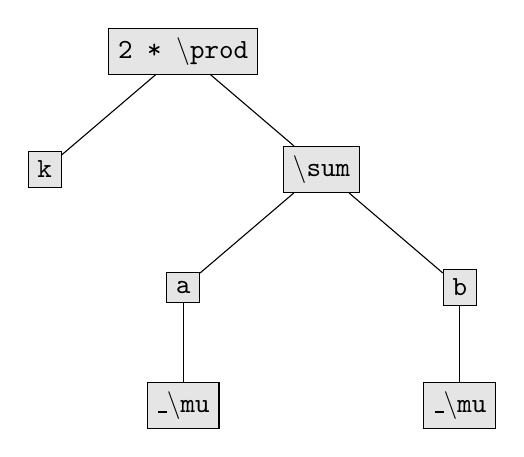
\begin{tikzpicture}[
		sibling distance=10em,
		every node/.style = {shape=rectangle, draw, align=center, fill=gray!20}]
		\node {\texttt{2 * \textbackslash prod}}
			child { node {\texttt{k}} }
			child { node {\texttt{\textbackslash sum}}
				child { node {\texttt{a}}
					child { node {\texttt{\_\textbackslash mu}} } }
				child { node {\texttt{b}}
					child { node {\texttt{\_\textbackslash mu}} } } };
	\end{tikzpicture}
\end{figure}

If the relation between this and the expression $2k(a_{\mu} + b_{\mu})$ is unclear then there is a good
explanation of how to build up these trees on the Mathematics StackExchange\footnote{
\url{https://math.stackexchange.com/a/369807}} and the Wikipedia article for binary trees\footnote{
\url{https://en.wikipedia.org/wiki/Binary_expression_tree}} although it should be remembered that operator nodes
in the Cadabra expression tree are not limited to two children.

Access to this tree in Python allows arbitrary manipulation of expressions. The tree can be traversed in
numerous ways, with \texttt{ExNode} objects providing an interface to the nodes in the tree. These both expose
various properties of the tree as well as methods which allow the insertion, modification and removal of nodes:
these methods are enumerated in Appendix \ref{app:exnode}. 

There are three main ways of obtaining references to nodes in the tree:
\begin{enumerate}[label=\textbf{\arabic*}.]
	\item \textbf{\texttt{Ex.top()}}
	
	The node representing the top node of a tree can be obtained by using the \texttt{top} method of a
	\texttt{Ex} object. From this, the tree can be further explored by using one of the \texttt{ExNode} methods
	which returns an iterator, for example
	\begin{lstcdb}
		for node in ex.top().children():
			print(node.name)
	\end{lstcdb}
	which for the expression above prints
	\begin{lstverb}
		k
		\sum
	\end{lstverb}

	\item \textbf{Name search}
	
	It is possible to iterate over nodes based on their name as in the following example:
	\begin{lstcdb}
		ex := <m>v_{\mu} v^{\mu} \gamma_{\rho \lambda} + T_{\rho \lambda}</m>;
		for node in ex[r'\mu']:
			node.name = r'\nu'
	\end{lstcdb}
	where the expression now reads $v_{\nu} v^{\nu} \gamma_{\rho \lambda} + T_{\rho \lambda}$
	\item \textbf{Whole tree traversal}
	
	The simplest traversal method is to visit the whole tree using a for loop:
	\begin{lstcdb}
		for node in ex:
			print(node.name)
	\end{lstcdb}
	For the expression above this prints
	\begin{lstverb}
		\prod
		k
		\sum
		a
		\mu
		b
		\mu
	\end{lstverb}
	This is known as \emph{preorder} iteration, i.e. each node is returned before its children are visited.	
\end{enumerate}


\subsection{Accessing property information}

In many cases, in order for a algorithm to work correctly we need to be able to query subexpressions to see
which properties they have assigned. This can be done using the \texttt{.get(ex)} method of a property which
returns the corresponding property object if it assigned to the expression or \texttt{None} otherwise. In the
following example this lets us check whether various objects are defined as coordinates:
\begin{lstcdb}
	<m>{t, x, y, z}</m>::Coordinate.
	Coordinate.get($t$);
	Coordinate.get($\phi$);
	for node in $x, r$.top().children():
		Coordinate.get(node);
\end{lstcdb}
\begin{lstverb}
	Property Coordinate attached to t.
	None
	Property Coordinate attached to x
	None
\end{lstverb}
Note that some properties, such as \texttt{Coordinate}, can be dependent upon their parent relationship, for
example the $t$ in $v_t$ is still a coordinate but the following returns \texttt{None}:
\begin{lstcdb}
	ex := <m>v_{t}</m>.
	for node in ex['t']:
		Coordinate.get(node);
\end{lstcdb}
	In this instance, we can pass the optional argument \verb|ignore_parent_rel=True| to allow Cadabra to make the
	match:
\begin{lstcdb}
	for node in ex['t']:
		Coordinate.get(node, ignore_parent_rel=True);
\end{lstcdb}
Many property object have extra methods which provide extra information, usually these are from attributes
passed when the property was declared. In the following example we can use this to see which values various
indices run over:
\begin{lstcdb}
	<m>{i, j, k, l}</m>::Indices(<m>cartesian, values={x,y,z}</m>).
	<m>{\mu, \nu, \rho, \lambda}</m>::Indices(<m>polar, values={r, \phi, \theta}</m>).
	ex := <m>x^{i}x^{i} + p_{\mu}p^{\mu}</m>.
	for node in ex:
		prop = Indices.get(node)
		if prop is not None:
			print(node.name, prop.values)
\end{lstcdb}
\begin{lstverb}
	i [x, y, z]
	i [x, y, z]
	\mu [r, \phi, \theta]
	\mu [r, \phi, \theta]
\end{lstverb}
To get a list of which extra methods a property defines you can use \verb|dir| or \verb|help| to list all the
methods it defines.

\subsection{Algorithms using \texttt{def}}

For almost all situations you are likely to come across, a simple definition of an algorithm using a Python
function will be sufficient. We already saw a bad example of this in the previous section with 
\verb|distribute_excluding|; lets rewrite that now to make it more conventional:
\begin{lstcdb}
	def distribute_excluding(ex, subex):
		substitute(ex, $@(subex) -> qqq$)
		distribute(ex)
		substitute(ex, $qqq -> @(subex)$)
		return ex
\end{lstcdb}
This is a simple routine which allows us to limit the effects of \verb|distribute| on an expression which can
be useful if there are some common factors containing sums which we want to preserve, for example in
Schwarzchild space-time where factors of $2M - r$ are common. Of course, this is a slightly na\"ive way of
writing this (it will cause unexpected behaviour in the event someone uses \texttt{qqq} as a variable name and
is limited to only allowing one expression to be excluded) but illustrates a common technique for writing
algorithms quite nicely: more complicated manipulations can often be produced simply by combining the
inbuilt algorithms like this to suit specific needs. 

\subsection{Algorithms using \texttt{@algo}}

A common technique for writing algorithms is to traverse the expression tree checking each node against a criteria and applying
a function to it if the criteria is satisfied. The entire collection of core algorithms is built in this manner and the pattern
is implemented in the \texttt{Algorithm} class. This is a abstract base class with two pure virtual methods: \verb|can_apply|
which implements the predicate checking if an operation can be applied to a tree node, and \verb|apply| which then carries out
the actual operation. 

The class itself is, however, usually not directly visible to users --- instead its behaviour is wrapped inside of a function
which takes care of iterating through the tree, calling \verb|can_apply| and \verb|apply|, and ensuring that the tree is in
a normalised state after the operation. In Python this wrapping is implemented with the \verb|@algo| decorator which
automatically converts the class into an appropriate function call. A very simple example is the following \verb|x_to_y|
algorithm. We first need to import the relevant objects from the \verb|cdb.utils.develop| library:  
\begin{lstcdb}
	from cdb.utils.develop import algo, Algorithm
\end{lstcdb} 
We then define a decorated class which inherits from \verb|Algorithm| and overrides the two virtual functions:
\begin{lstcdb}
	@algo
	class x_to_y(Algorithm):
		def can_apply(self, node):
			return node.name == 'x'
		def apply(self, node):
			node.name = 'y'
			return result_t.changed
\end{lstcdb}
The predicate in this instance simply checks the name of the node, but in all cases it should return a boolean type. Any node
for which the result is \verb|False| is skipped and so the \verb|apply| method can make assumptions about node it receives as
a parameter based on this. In this case, it knows that it can change the name to \texttt{y}. The return value of the 
\verb|apply| method is of type \verb|result_t| which should take on the value \texttt{changed} if some transformation was
applied, \texttt{error} if some error occurred inside the method or \texttt{unchanged} if \verb|apply| ended up making no
modifications to the tree. \verb|apply| \emph{must} return a \verb|result_t| or an exception will be raised when the algorithm
is called that the function signature is incorrect.

The \verb|@algo| decorator converts this into a function so we call this algorithm as any other algorithm in Cadabra:
\begin{lstcdb}
	x_to_y($x + y$)
\end{lstcdb}
\begin{lstverb}
	2y
\end{lstverb}
Notice that various cleanup routines are automatically called after the algorithm is applied which simplifies the expression
from $y + y$ into $2y$. 

The function is also given the optional keyword arguments \verb|deep|, \verb|repeat| and \verb|depth| with the same behaviour
as the core algorithms.

\subsubsection*{Stateful algorithms}
Sometimes it is necessary for an algorithm to be stateful, that is either be passed extra information through parameters when
it is called or to retain some information between various calls to \verb|apply|. This can be done by overriding the 
\verb|__init__| method of the class; any arguments passed to the function call (other than \verb|deep|, \verb|repeat| and
\verb|depth|) are forwarded onto this constructor.  Let's use this to extend our \verb|x_to_y| algorithm into one where we can
specify other values for \verb|x| and \verb|y|:
\begin{lstcdb}
	@algo
	class x_to_y(Algorithm):
		def __init__(self, ex, x='x', y='y'):
			Algorithm.__init__(self, ex)
			self.x = x
			self.y = y
		def can_apply(self, node):
			return node.name == self.x
		def apply(self, node):
			node.name = self.y
			return result_t.changed
\end{lstcdb}
We can now use this as a `y-to-x' algorithm too:
\begin{lstcdb}
	x_to_y($x + y$, x='y', y='x');
\end{lstcdb}
\begin{lstverb}
	2x
\end{lstverb}
Its important to ensure that the first argument to the \verb|__init__| method is the \verb|Ex| object on which the algorithm
is called, and to remember to call the base \verb|Algorithm| constructor too.

\subsubsection*{Functional shortcut}
For simple algorithms such as our \verb|x_to_y| example here, instead of defining an entire class we can also just supply
\verb|@algo| with a function and it will automatically generate the class definition using the function body for the
\verb|apply| method:
\begin{lstcdb}
	@algo
	def x_to_y(node):
		if node.name == 'x':
			node.name = 'y'
			return result_t.changed
		return result_t.unchanged
\end{lstcdb}
Note that it is not possible to create a stateful algorithm using this method, the definition using a class as shown above must
be used if this is desired.
Anoher drawback to this approach is that the predicate is now inside the body of \verb|apply| which results in slightly less
efficient code being produced, but this is negligible for simple algorithms such as this for which the shorthand is intended.
If this does become a concern, it is also possible to supply \verb|algo| with a verb|pred| parameter which it will use as the
body for \verb|can_apply| eliminating the need to perform this check inside the function body:
\begin{lstcdb}
	@algo(pred=lambda node: node.name == 'x')
	def x_to_y(node):
		node.name = 'y'
		return result_t.changed
\end{lstcdb}
This produces code which is identical to the first class definition we discussed above. 

\subsection{Documenting algorithms}

As notebooks can be imported from other notebooks using Python's \texttt{import} statement, many Cadabra packages are written
in notebooks which allows the documentation to be provided in accompanying \LaTeX{} cells. In order to format this documentation
the \texttt{algorithm} command is provided which takes two arguments: the signature of the algorithm's function call and a
brief description of its use and application. 

The signature should contain the types of all the arguments and the return value using Python's type hinting style, for 
example a function which takes a \texttt{Ex} object and a \texttt{int} and returns a \texttt{Ex} might be documented like
\begin{lstlatex}
\algorithm{my_algo(ex: Ex, n: int) -> Ex}{Does some transformation to \texttt{ex} which involves \texttt{n}}
\end{lstlatex}
\fcolorbox{gray!50}{white}{%
	\begin{minipage}{\textwidth}
		\vspace{1mm}
		\algorithm{my_algo(ex: Ex, n: int) -> Ex}{Does some transformation to \texttt{ex} which involves \texttt{n}}
	\end{minipage}	
}

\section{Writing Cadabra algorithms in C++}

Although one of the greatest strengths of Cadabra is how easy it is to extend using Python, efficiency can sometimes cause 
issues either on very large expressions or when algorithms reach a certain level of complexity and are hindered by the
Python interpreted runtime. In these instances, writing the algorithm in C++ is almost certainly the necessary solution. It is
not a common occurrence for users to contribute C++ algorithms and so no specific functionality has been developed in order to
facilitate the writing of external libraries and so it is necessary to build Cadabra from source and develop the algorithm
inside the core codebase, however Cadabra always welcomes community contributions and if the algorithm proves to be useful then
it may well be included in a future release of Cadabra.

There are two ways of placing a C++ algorithm into Cadabra: either by extending the list of core algorithms, or by placing the
code in a library package. In either instance, the first step is to get the Cadabra code base from github
\footnote{\url{https://github.com/kpeeters/cadabra2}} and follow the build instructions for your OS. The next optional
(but recommended especially if you are planning of submitting a pull request) is to set up a new git branch to perform your
development on. 

\subsection{Writing a core algorithm}

As with the \verb|@algo| style of algorithm definition in Python, the core algorithms in C++ all derive from the C++
\verb|Algorithm| class. First, you should create a header and source file where the code for you algorithm will live. As with
the previous example, we will create the simple \verb|x_to_y| algorithm and so we create the files 
\verb|core/algorithms/x_to_y.hh| and \verb|core/algorithms/x_to_.cc|. We also need to tell CMake about the new source file by
adding a line to the \verb|ALGORITHM_SRC_FILES| variable in \verb|core/CMakeLists.txt|:
\begin{lstverb}
SET(ALGORITHM_SRC_FILES
   algorithms/canonicalise.cc
   algorithms/collect_components.cc
   algorithms/collect_factors.cc
   ...
   algorithms/unwrap.cc
   algorithms/unzoom.cc
   algorithms/untrace.cc
   <add>algorithms/x_to_y.cc</add>
   algorithms/vary.cc
   algorithms/young_project.cc
   algorithms/young_project_product.cc
)
\end{lstverb}
Next we need to define the \verb|x_to_y| class in the header file \verb|core/algorithms/x_to_y.hh| we just created:
\begin{lstcpp}
	#pragma once
	#include <Algorithm.hh>
	
	namespace cadabra {
		class x_to_y : public Algorithm {
			public:
				x_to_y(const Kernel& kernel, Ex& ex);
	
				bool can_apply(Ex::iterator it) override;
				result_t apply(Ex::iterator& it) override;
			};
		}
\end{lstcpp}
This should be fairly understandable, the signatures of all the class methods must be the same as in this example but you
may add more parameters to the constructor after the \verb|Ex| reference (as we will do later). We can now move on to the
implementation which goes into \verb|core/algorithms/x_to_y.cc|. We start by importing the header and for convenience 
pulling \verb|cadabra| into the global namespace:
\begin{lstcpp}
	#include "algorithms/x_to_y.hh"
	
	using namespace cadabra;
\end{lstcpp}
For the simple algorithm we are writing, we will simply forward the constructor arguments onto the \verb|Algorithm| constructor:
\begin{lstcpp}
	x_to_y::x_to_y(const Kernel& kernel, Ex& ex)
		: Algorithm(kernel, ex)
		{
	
		}
\end{lstcpp}
Next we write in our implementation of \verb|can_apply|. This is a very straightforward function, the only thing to keep in 
mind is that node names in Cadabra are interned and so to access the \verb|std::string| representation of them they must
be dereferenced:
\begin{lstcpp}
	bool x_to_y::can_apply(Ex::iterator it)
		{
		return *it->name == "x";
		}
\end{lstcpp}
The last bit of code we need to write in this file is the implementation of \verb|apply|. Again, as the strings are interned
instead of assigning a string we must query the global \verb|name_set| for an iterator and store the value this returns to us:
\begin{lstcpp}
	Algorithm::result_t x_to_y::apply(Ex::iterator& it)
		{
		it->name = name_set.insert("y").first;
		return result_t::l_applied;
		}
\end{lstcpp}
It is also worth mentioning that the \verb|result_t| names differ between the Python and C++ interfaces; whereas before we
used \verb|changed| and \verb|unchanged| in C++ we use \verb|l_applied| and \verb|l_no_action| respectively.

The final step we need to perform is the Python interfacing code in \verb|core/pythoncdb/py_algorithms.cc|. We first add our
header file to the list of includes at the top:
\begin{lstcpp}
	...
	#include "../algorithms/unwrap.hh"
	#include "../algorithms/unzoom.hh"
	#include "../algorithms/untrace.hh"
	<add>#include "../algorithms/x_to_y.hh"</add>
	#include "../algorithms/vary.hh"
	#include "../algorithms/young_project.hh"
	#include "../algorithms/young_project_product.hh"
	#include "../algorithms/young_project_tensor.hh"
	...
\end{lstcpp}
The final step before building is then the actual binding code. This is the least intuitive part of the process, but most of
the technical details are hidden and all that needs to be done is to call \verb|def_algo| templated against the
\verb|x_to_y| class. You can add this line to the end of the list of \verb|def_algo| declarations in the 
\verb|init_algorithms| function:
\begin{lstcpp}
	void init_algorithms(py::module& m)
		{
		pybind11::enum_<Algorithm::result_t>(m, "result_t")
		.value("checkpointed", Algorithm::result_t::l_checkpointed)
		...
		def_algo_preorder<meld, bool>(m, "meld", true, false, 0, py::arg("project_as_sum") = false);
		<add>def_algo<x_to_y>(m, "x_to_y", true, false, 0);</add>
		}
\end{lstcpp}
The first argument is a handle to the \verb|cadabra2| Python module and the second is the name of the function on the 
Python side, this should be the same as the C++ name to avoid confusion. The next three parameters are the default values of
the \verb|deep|, \verb|repeat| and \verb|depth| parameters but these can be changed in Python when calling the algorithm
by using the optional keyword arguments.

It's now time to build Cadabra again and try out the new algorithm. The algorithm will be imported into the global scope at
launch:
\begin{lstcdb}
	x_to_y($x + y$);
\end{lstcdb}
\begin{lstverb}
	2y
\end{lstverb}

\subsubsection*{Adding extra constructor parameters}

As with our \verb|x_to_y| function from the Python section, a natural extension would be to allow users to provide values of
\verb|x| and \verb|y|. This only requires a few alterations to the code we have written: first the constructor must be 
altered to take the new parameters and the class definition extended to include the two new variables \verb|x| and \verb|y|. We will store these as interned strings and so we declare them as \verb|nset_t::iterator| variables. The new class definition in 
\verb|x_to_y.hh| now looks as follows
\begin{lstcpp}
	class x_to_y : public Algorithm {
		public:
			x_to_y(const Kernel& kernel, Ex& ex, const std::string& x, const std::string& y);

			bool can_apply(Ex::iterator it) override;
			result_t apply(Ex::iterator& it) override;

		private:
			nset_t::iterator x, y;
		};
\end{lstcpp}
Moving onto \verb|x_to_y.cc|, we now also change the constructor signature here and initialise \verb|x| and \verb|y|:
\begin{lstcpp}
	x_to_y::x_to_y(const Kernel& kernel, Ex& ex, const std::string& x, const std::string& y)
		: Algorithm(kernel, ex)
		, x(name_set.insert(x).first)
		, y(name_set.insert(y).first)
		{
	
		}
\end{lstcpp}
The \verb|can_apply| and \verb|apply| function definitions also need to use the stored values instead of the hardcoded
values of \verb|x| and \verb|y|:
\begin{lstcpp}
	bool x_to_y::can_apply(Ex::iterator it)
	{
		return it->name == x;
	}
	
	Algorithm::result_t x_to_y::apply(Ex::iterator& it)
	{
		it->name = y;
		return result_t::l_applied;
	}
\end{lstcpp}
Almost done: just one more line to change, the Python binding code. In order to make Python aware that the function now takes
two extra arguments, we need to add the types of these these extra arguments to the list of template parameters of 
\verb|def_algo|. We also need to give these extra arguments Python names, which is done by adding a \verb|py::arg| object
parameter onto the end of the list of \verb|def_algo|'s parameters for each argument. The final binding code should look like
this:
\begin{lstcpp}
	def_algo<x_to_y, const std::string&, const std::string&>(
		m, "x_to_y", true, false, 0, 
		py::arg("x"), py::arg("y"));
\end{lstcpp}
After building, this is now accessible from Cadabra:
\begin{lstcdb}
	x_to_y($x + y$, 'y', 'x')
\end{lstcdb}
\begin{lstverb}
	2x
\end{lstverb}

\subsection{Writing a package algorithm}

Recently, additions to the binding code have allowed the possibility of creating Cadabra packages in C++. There is currently
only support in the build system for creating libraries for the builtin \verb|cdb.*| libraries. This can be used to refactor
algorithms contained in these libraries which are currently implemented in Python into C++ routines, or to provide `non-core'
functionality in an easily accessible location without polluting the global namespace.

It is recommended that the C++ library is prefixed with an underscore, and the relevant functions, classes or other definitions
which it provides imported into a Cadabra notebook with the documentation attached there. Therefore, if we wanted to create
a \verb|cdb.core.subs| module for our \verb|x_to_y| algorithm, we would create the C++ module \verb|cdb.core._subs| and then
have a notebook \verb|cdb.core.subs| with the contents
\begin{lstlatex}
\algorithm{x_to_y(ex: Ex) -> Ex}{Renames all nodes names x to y}
\end{lstlatex}
\begin{lstcdb}
from cdb.core._subs import x_to_y
\end{lstcdb}

To create the package, we first need to make a file \verb|core/packages/cdb/core/_subs.cc|. To make the build system aware
of the package, we need to add it to the \verb|COMPILED_PACKAGES| variable in the build script located at
\verb|core/packages/CMakeLists.txt|:
\begin{lstverb}
set(COMPILED_PACKAGES
  core/_component.cc
  utils/_algorithm.cc
  <add>core/_subs.cc</add>
  )
\end{lstverb}
The contents of the file \verb|_subs.cc| is very similar to the code used for implementing a core algorithm. We begin by
importing the functionality from the \verb|py_algorithms.hh| header which will also give us access to the \verb|Algorithm|
class, and we will then bring it into scope by importing all the names from the \verb|cadabra| namespace:
\begin{lstcpp}
	#include "pythoncdb/py_algorithms.cc"
	
	using namespace cadabra;
\end{lstcpp}
We can then implement the \verb|x_to_y| class as before, here we use inline function definitions for brevity:
\begin{lstcpp}
	class x_to_y : public Algorithm {
		public:
			x_to_y(const Kernel& kernel, Ex& ex)
				: Algorithm(kernel, ex)
				{
	
				}
	
			bool can_apply(Ex::iterator it) override
				{
				return *it->name == "x";
				}
	
			result_t apply(Ex::iterator& it) override
				{
				it->name = name_set.insert("y").first;
				}
		};
\end{lstcpp}
Finally we create the Python module itself using the \verb|PYBIND11_MODULE| macro. The first argument must match the filename
as this will be the name of the module, the second argument can be any valid identifier. We can then call \verb|def_algo|
just as before:

\begin{lstcpp}
	PYBIND11_MODULE(_subs, m)
	{
		def_algo<x_to_y>(m, "x_to_y", true, false, 0);
	}
\end{lstcpp}
After building, this will now be available to import into Cadabra. Assuming we have also created the \verb|subs| notebook as
described above, we can now call the \verb|x_to_y| from there:
\begin{lstcdb}
	x + y
\end{lstcdb}
\begin{lstverb}
	2y
\end{lstverb}
Extending this to the alternate form of \verb|x_to_y| with extra arguments is done exactly as for the case when writing a 
core algorithm was discussed.

Circling back to the very beginning of this tutorial, it is of course also possible to create a function which does this
by accepting and returning a \verb|Ex_ptr| (a convenience typedef for the \verb|Ex| pointer type exposed to Python):
\begin{lstcpp}
	Ex_ptr x_to_y(Ex_ptr ex)
		{
		for (Ex::iterator beg = ex->begin(), end = ex->end(); beg != end; ++beg) {
			if (*beg->name == "x")
				beg->name = name_set.insert("y").first;
			}
		return ex;
		}
\end{lstcpp}
with the binding code
\begin{lstcpp}
	m.def("x_to_y", x_to_y);
\end{lstcpp}


\appendix

\newpage
\section{Reserved node names}
\label{app:nodenames}

More information on the behaviour of these nodes can be found in the Cadabra documentation.

\begin{table}[H]
	\centering
	\renewcommand{\arraystretch}{1.5}
	\begin{tabular}{|c|c|c|}
	\hline
	\rowcolor[HTML]{C0C0C0} 
	Symbol & Node name & Brief description    \\ \hline
	$\times$ & \verb|\prod| 
		& Product of children\\ \hline
	$+$ & \verb|\sum| 
		& Sum of children  \\ \hline
	$\oplus$ & \verb|\oplus| 
		& Tensor sum of children \\ \hline
	$\frac{x}{y}$ & \verb|\frac| 
		& Quotient of children (internal use only)  \\ \hline
	$,$ & \verb|\comma| 
		& List of children as independent expressions \\ \hline
	$\rightarrow$ & \verb|\arrow| 
		& Substitution rule from first child to second \\ \hline
	$\cdot$ & \verb|\inner| 
		& Inner product of children \\ \hline
	$x^y$ & \verb|\pow| 
		& First child to power of second child \\ \hline
	$\int$ & \verb|\int| 
		& Integral of first child w.r.t second child \\ \hline
	$=$ & \verb|\equals| 
		& First child equals second child \\ \hline
	$\neq$ & \verb|\unequals| 
		& First child does not equal second child \\ \hline
	$[a, b]$ & \verb|\commutator| 
		& Commutator between two children \\ \hline
	$\{a, b\}$ & \verb|\anticommutator| 
		& Anticommutator between  two children \\ \hline
	$\left\{\begin{aligned}\square_t &= \cdots \\ &\cdots\end{aligned}\right.$ & \verb|\components|
		& Component values of free indices \\ \hline
	$\wedge$ & \verb|\wedge| 
		& Wedge product of children \\ \hline
	$x\quad\text{with}\quad y$ & \verb|\conditional| 
		& First child as pattern which holds under second child \\ \hline
	$<$ & \verb|\less| 
		& First child is less than second child\\ \hline
	$>$ & \verb|\greater| 
		& First child is greater than second child\\ \hline
	$(A+B+C)_\mu$ & \verb|\indexbracket|
		& First child is an object with indices given by the remaining children \\ \hline
	$\cdots$ & \verb|\ldots|
		& Suppressed terms \\ \hline
	
	\end{tabular}
\end{table}

\newpage
\section{\texttt{ExNode} methods and properties}
\label{app:exnode}

\renewcommand{\descriptionlabel}[1]{\hspace{\labelsep}\textbf{\texttt{#1}}}
\subsection{Properties}
\begin{description}
	\item[name] 
		The name of the current node
	\item[parent\_rel] 
		The relationship of the current node to its parent
	\item[multiplier]
		The rational multiplier attached to the current node
\end{description}
\subsection{Methods}
\begin{description}
	\item[args()]
		Return an iterator over all arguments of the current node
	\item[append\_child(other)] 
		Append a \texttt{Ex} or \texttt{ExNode} as a child of the current node
	\item[children()]
		Return an iterator over all children of the current node
	\item[compare(other, use\_props, ignore\_parent\_rel] 
		Compare to another \texttt{ExNode}. Returns a \texttt{match\_t} object.
	\item[erase()] 
		Erase the current node
	\item[ex()] 
		Return a copy of the current node as a \texttt{Ex} object
	\item[factors()]
		Return an iterator over all factors at the level of the current node
	\item[free\_indices()]
		Return an iterator over all free indices of the current node
	\item[indices()]
		Return an iterator over all indices of the current node
	\item[insert(other)]
		Insert a \texttt{Ex} or \texttt{ExNode} object in front of the current node
	\item[own\_indices()]
		Return an iterator over all indices of the current node which are not inherited from child nodes
	\item[replace(ex)]
		Replace the current node with a \texttt{Ex} object
	\item[terms()]
		Return an iterator over all terms at the level of the current node
\end{description}

\end{document}
